\documentclass[letterpaper, 10 pt, conference]{article} 
\usepackage[english]{babel}
\usepackage{amsmath,amssymb,amscd,amsthm} % variety of useful math macros
\usepackage[inner=1.5 cm, outer = 1.5 cm, top=1 cm, bottom = 1.5 cm]{geometry}
\usepackage{subcaption}
%For inserting graphics
\usepackage{graphicx}
\usepackage[dvipsnames]{xcolor}
\usepackage{listings}
\usepackage[utf8]{inputenc}
\usepackage{hyperref}
\usepackage{array, multirow}
\usepackage{lipsum}
\usepackage{natbib}
\usepackage[normalem]{ulem}


\bibliographystyle{abbrvnat}

\newtheorem{thm}{Theorem}
\newtheorem{prop}{Proposition}
\newtheorem{lemma}{Lemma}
\newtheorem{ex}{Exercise}
\newtheorem{exm}{Example}
\newtheorem{defn}{Definition}

\newcommand\E{\ensuremath{\mathbb{E}}}
\newcommand\N{\ensuremath{\mathbb{N}}}
\renewcommand{\P}{\ensuremath{\mathbb{P}}}
\newcommand\Q{\ensuremath{\mathbb{Q}}}
\newcommand\R{\ensuremath{\mathbb{R}}}
\newcommand\Z{\ensuremath{\mathbb{Z}}}

\newcommand\var[1]{\, \mathrm{Var} \left( #1 \right)}

\newcommand\pr[1]{\, \mathbb{P} \left( #1 \right)}

\newcommand\cov[1]{\, \mathrm{Cov} \left( #1 \right)}

\newcommand\expec[1]{\, \mathbb{E} \left\lbrack #1 \right\rbrack}

\title{Law of large numbers
}
\date{December 1, 2020}

\hypersetup{
	colorlinks=true,
	linkcolor=blue,
	filecolor=magenta,      
	urlcolor=blue,
	citecolor=MidnightBlue
}

\author{Gerardo {\textsc{Palafox}}}


\begin{document}
\maketitle
\begin{abstract}
	In this work, the law of large numbers is presented, along some applications of the same.
\end{abstract}
\section{Introduction}
 Two theorems will be given, known as the weak and strong law of large numbers. Both of the statements, as well as the definitions preceding it, can be found in the work of \citet{Casella_Berger_2002}. 
 
\begin{defn}\label{defn:converge_probability}
	A sequence of random variables $X_1, X_2, \dots$, converges in probability to a random variable $X$ if, for every $\varepsilon > 0$, 
	\begin{equation}
		\lim_{n \rightarrow \infty} \pr{|X_n - X| \geq \varepsilon } = 0 \; \text{ or, equivalently } \; \lim_{n \rightarrow \infty} \pr{|X_n - X| < \varepsilon } = 1
	\end{equation}
\end{defn}

\begin{defn}\label{defn:converge_as}
	A sequence of random variables $X_1, X_2, \dots$, converges almost surely to a random variable $X$ if, for every $\varepsilon > 0$, 
	\begin{equation}
		\pr{\lim_{n \rightarrow \infty} |X_n -X| < \varepsilon} = 1
	\end{equation}
\end{defn}

\begin{thm}[Weak law of large numbers]\label{thm:weak_lln}
	Let $X_1, X_2, \dots$ be independent, identically distributed random variables with $\expec{X_i} = \mu$ and $\var{X_i} = \sigma^2 < \infty$. Then, $\bar{X_n} = (1/n) \sum_{i = 1}^{n} X_i$ converges in probability to $\mu$.
\end{thm}

\begin{thm}[Strong law of large numbers]\label{thm:strong_lln}
	Let $X_1, X_2, \dots$ be independent, identically distributed random variables with $\expec{X_i} = \mu$ and $\var{X_i} = \sigma^2 < \infty$. Then, $\bar{X_n} = (1/n) \sum_{i = 1}^{n} X_i$ converges almost surely to $\mu$.
\end{thm}

\section{Renewal processes}
One of the many applications of the law of large numbers is in a kind of stochastic process called renewal processes. The contents of this section can be found in the book of \citet{lawler_2006}.

\begin{defn}
	Let $T_1, T_2, \dots$ be independent, identically distributed, non-negative random variables with distribution $F(x)$. The renewal process associated with $\lbrace T_i \rbrace$ is the process that counts the number of events that have occurred by time $t$. More precisely, the renewal process $N_t$ is defined by 
	\begin{equation}
		N_t = \begin{cases}
		0 & t < T_1; \\
		\max\lbrace n : T_1 + \dots + T_n \leq t\rbrace &  \text{ else.}
		\end{cases}
	\end{equation}
\end{defn}
The random variables $T_i$ are thought of as being the lifetimes of a component, or as the times between occurrences of some event. Time 0 is assumed as the beginning of a lifetime. The random variables $T_i$ are assumed to have finite, positive mean $\mu = \expec{T_i}$.

\begin{exm}\label{exm:poisson}
	Consider the Poisson process with waiting times $T_1, T_2, \dots$. These are independent, exponential random variables with parameter $\lambda$ and $N_t$ is the Poisson process.
\end{exm}

\begin{exm}\label{exm:queue}
Consider a queue with a single server where customers arrive according to a Poisson process with rate $\lambda$. Assume the service times for customers are independent, identically distributed random variables with mean $\mu$. Let $Y_t$ denote the number of people in the queue at time $t$.  Let 
\begin{align}
R_1 = \inf \lbrace t > 0 : Y_t = 1\rbrace, \\
S_1 = \inf\lbrace t > 0 : Y_{R_1 + t} = 0\rbrace, \\
T_1 = R_1 + S_1,
\end{align}
and for $i > 1$,
\begin{align}
R_i = \inf \lbrace t > 0 : Y_{T_1 + \dots + T_{i-1} +t} = 1\rbrace, \\
S_i = \inf\lbrace t > 0 : Y_{T_1 + \dots + T_{i-1} + R_i + t} = 0\rbrace, \\
T_i = R_i + S_i.
\end{align}
The time represented by $R_i$ can be thought of as idle times, and the time represented by $S_i$ as the busy times. The random variables $T_1, T_2, \dots$ give rise to a renewal process $N_t$. 
\end{exm}

Using the Strong Law of Large Numbers (Theorem \ref{thm:strong_lln}), the following analogue of the law of large numbers for renewal processes can be derived:

\begin{prop}
	For a renewal process $N_t$, with probability one,
	\begin{equation}
		\lim_{t \rightarrow \infty} \frac{N_t}{t} = \frac{1}{\mu}.
	\end{equation}
\end{prop}

A Poisson process (see Example \ref{exm:poisson}) was simulated\footnote{The code, as well as this report, can be found in \url{https://github.com/palafox794/AppliedProbabilityModels/tree/master/Assignment13}.} with R version 4.0.0 in a Jupyter notebook \citep{R, jupyter}. In Figure \ref{fig:lln} it is observed how $N_t /t \rightarrow 1/\mu$ as $t$ grows.

\begin{figure}
	\centering
	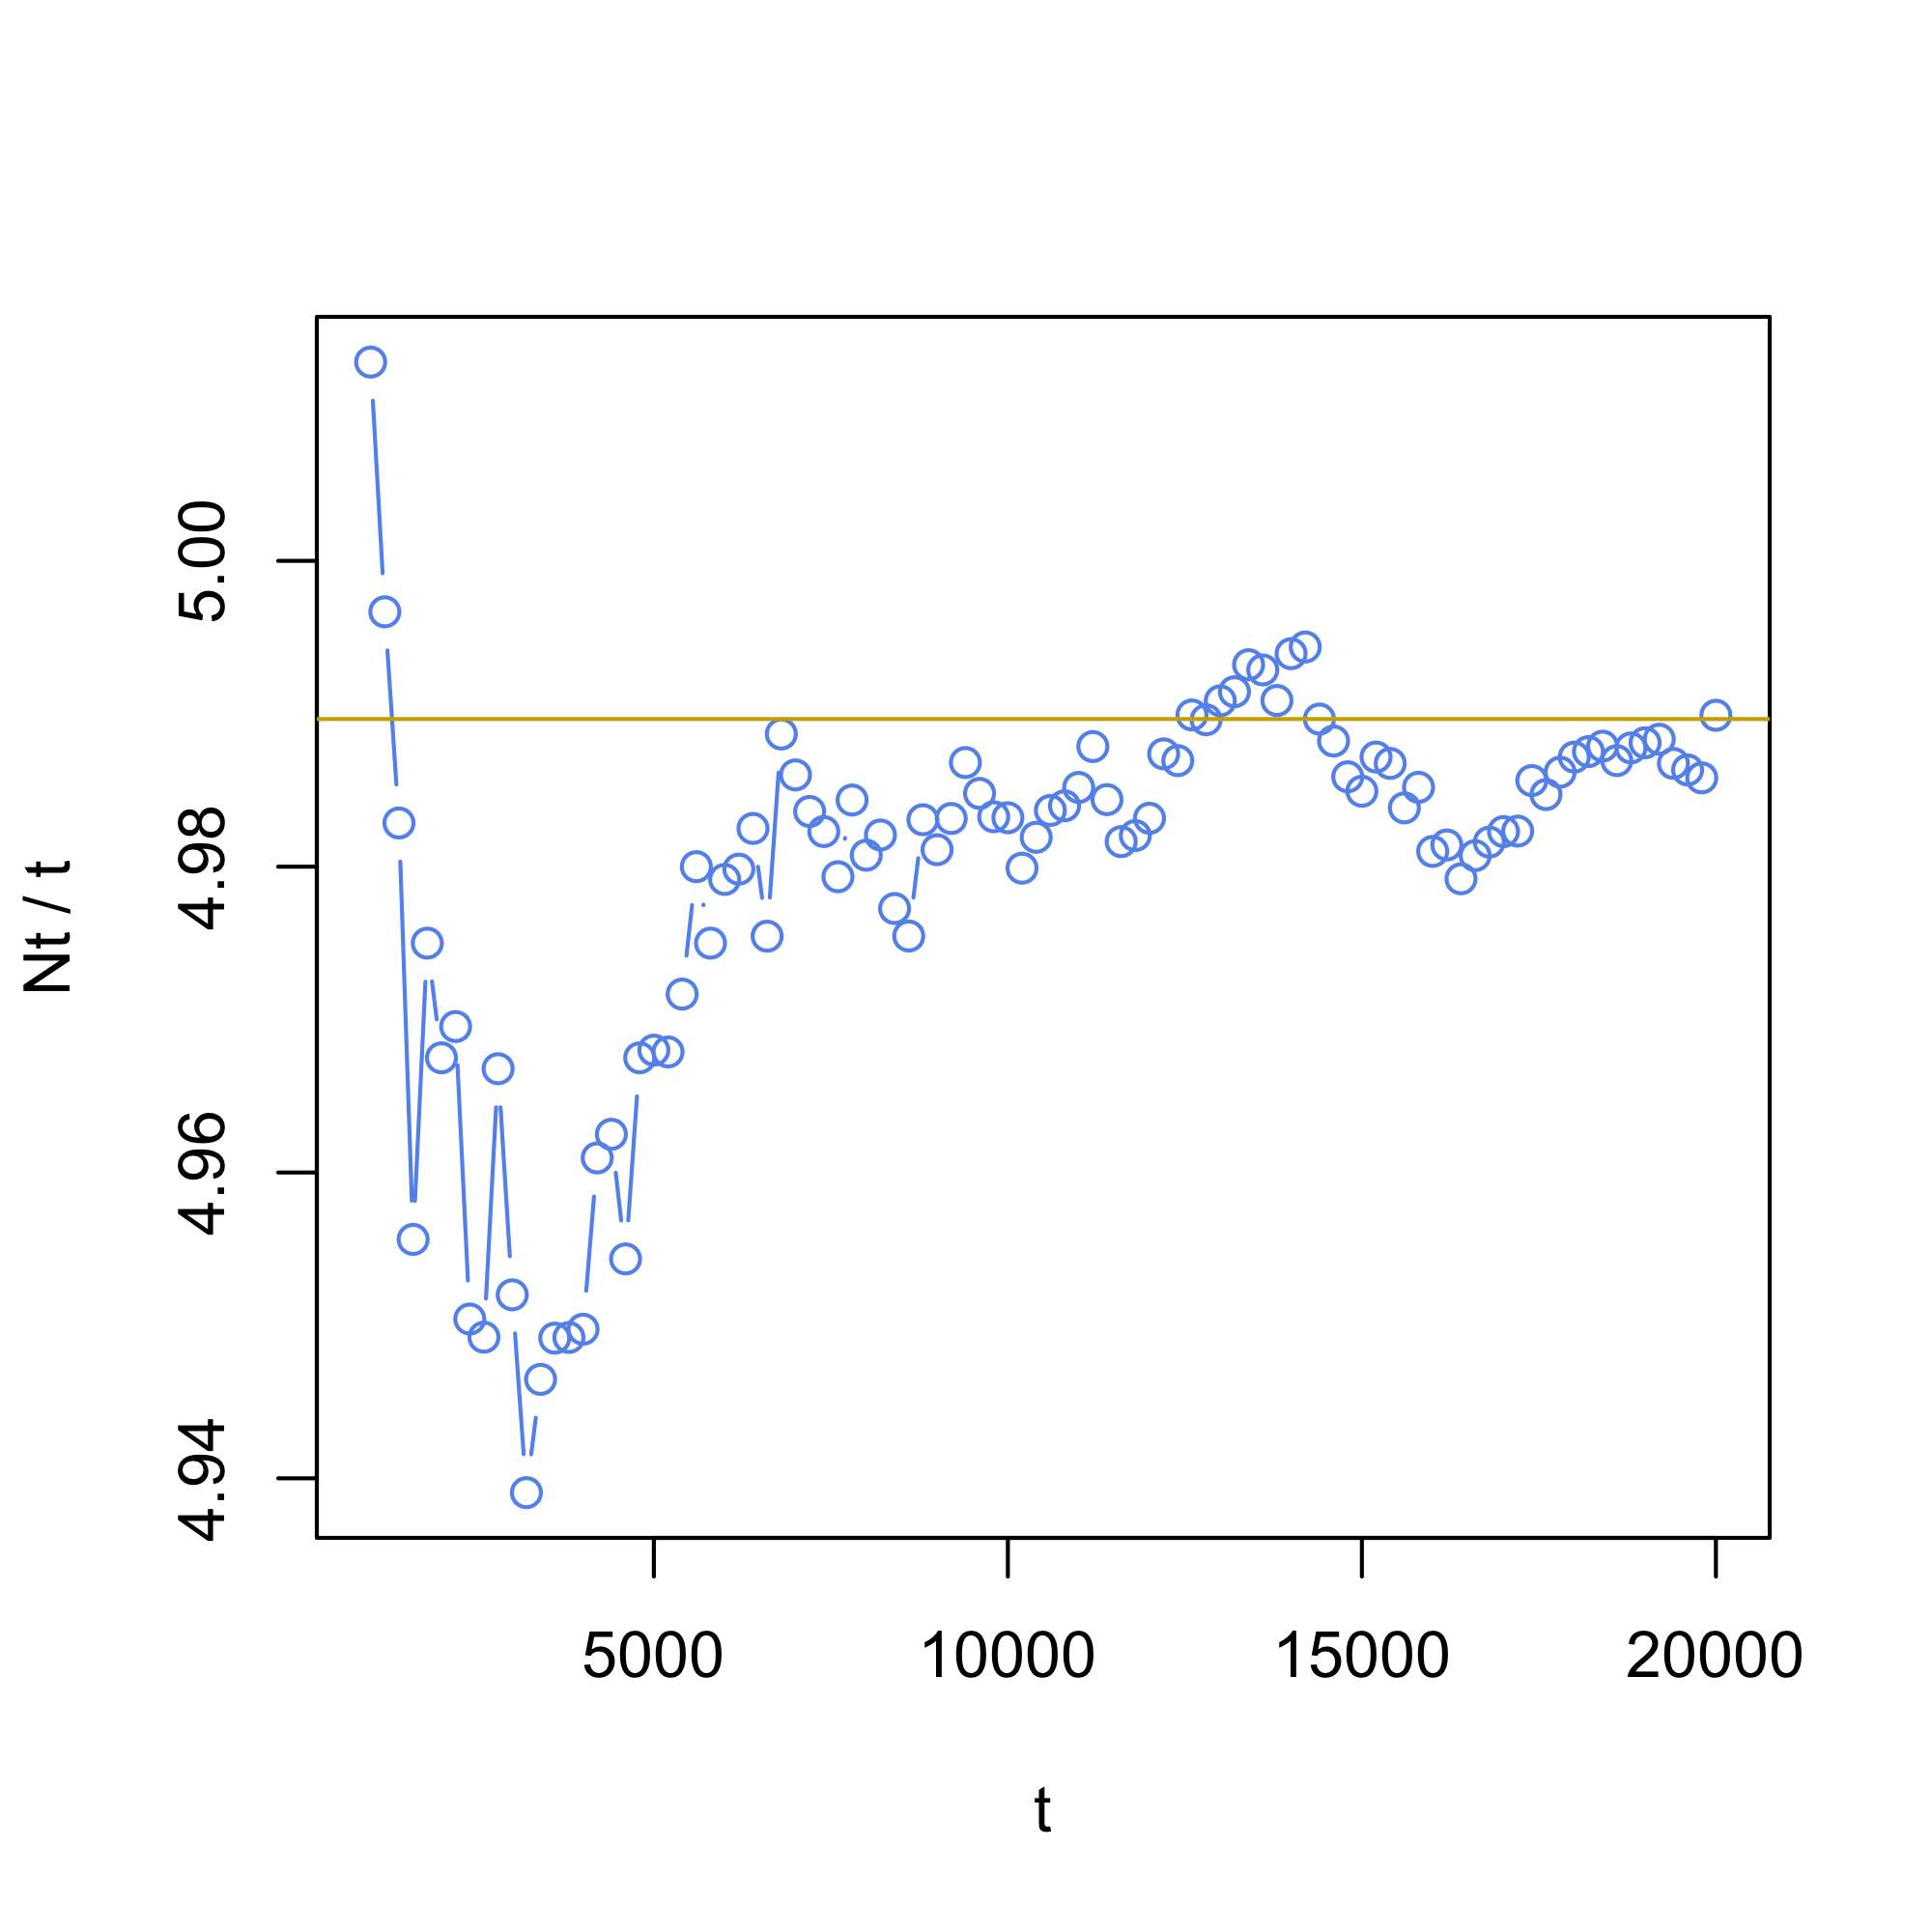
\includegraphics[width = .5 \linewidth]{lln.png}
	\caption{In blue, the value of $N_t / t$. In gold, the value $1/\mu$.}
	\label{fig:lln}
\end{figure}
%%%%%%%%%%%%%%%%%%%%%%%%%%%%%%%%%%%%%%%%%%%%%%%%%%%%%%%%%%%%%%%%%%%%%%%%%%%%%%%%

\section{Epidemics on networks}
In the work of \citet{janson2014law}, a law of large numbers is established for an epidemic process on a random graph. In particular, a random graph with a given degree sequence is considered. Given the graph, the epidemic evolves as a continuous-time Markov chain \citep{Liggett_2010} where each infectious vertex recovers at rate $\rho \geq 0$ and also infects each susceptible neighbor at a rate $\beta > 0$. The graph has $n$ vertices, of which initially $n_S, n_I, n_R$ are susceptible, infectious and recovered respectively. It is assumed the fractions of initially susceptible, infectious and recovered vertices converge to some $\alpha_S, \alpha_R, \alpha_I \in [0,1]$, with $\alpha_S > 0$. Additionally, it is assumed the degree of a randomly chosen susceptible vertex converges to a probability distribution $(p_k)_{k=0}^{\infty}$, that is, 
\begin{equation}
	n_{S,k} / n \rightarrow p_k,
\end{equation}
where $n_{S,k}$ is the number of susceptible vertices of degree $k$. Furthermore, the average degree over all vertices converges to $\mu > 0$. Let $S_t, I_t, R_t$ be the number of susceptible, infectious and recovered vertices at time $t$, and $T_0$ the time in which the fraction of susceptible individuals has fallen from about $\alpha_S$ to some fixed smaller $s_0$. \citet{janson2014law} prove that when the quantity
\begin{equation}
	R_0 := \left( \frac{\beta}{\beta + \rho}\right) \left( \frac{\alpha_S}{\mu} \right) \sum_{k = 0}^{\infty} (k-1) k p_k,
\end{equation}
interpreted as the basic reproduction number of the epidemic, is greater than one, then for every $\varepsilon > 0$,
\begin{equation}
	\pr{T_0 = \infty \text{ and } S_0 - S_\infty > \varepsilon n} \rightarrow 0.
\end{equation}
This represents a small outbreak. However, it is also proved that if $T_0 < \infty$, the outbreak is large.

\subsection{Vaccination}
In their work, \citet{janson2014law} also study the effects of different vaccination strategies. A perfect vaccine is assumed, so a vaccinated vertex never becomes infected and in practice behaves as recovered. It is assumed each initially susceptible vertex of degree $k$ is vaccinated with probability $\pi_k \in [0,1)$, independently of the others. As an example, consider the \textit{uniform vaccination} strategy. Here, every susceptible vertex is vaccinated with the same probability $v \in [0, 1)$, independently of all the others. Using the law of large numbers, it is proven that $V/n_S$ converges in probability to $v$, where $V$ is the total number $V$ of vaccinations. 

%%%%%%%%%%%%%%%%%%%%%%%%%%%%%%%%%%%%%%%%%%%%%%%%%%%%%%%%%%%%%%%%%%%%%%%%%%%%%%%%
\bibliography{ref}

\end{document}
